
\documentclass[12pt]{article}
\usepackage[a4paper, total={6.5in, 9in}]{geometry}
\usepackage{import}

\import{./}{macros}


\title{
    % UW Mech/Tron Eng Logo
    
\includegraphics[width=\linewidth]{resources/uwaterloo_mechanical_and_mechatronics_engineering/UWaterloo_Mechanical_Mechatronics_Eng_Logo_horiz_rgb.png}
    \\[1cm]
    \underline{\bf{ME 303 - Collapsing Vacuum Bubble ODEs}}
}
\author{
    Austin W. Milne\\
    Japmeet Brar\\
    Joshua Selvanayagam\\
    Kevin Chu
}
\date{March 16, 2022}


\begin{document}
\pagenumbering{gobble}
\maketitle
\vfill
\begin{abstract}
    Project 1 report for ME 303 in Winter 2022. Using numerical ODE solutions to model the collapse and rebound of underwater vacuum bubbles. Project source code and report available at:
    \underline{\url{https://github.com/Awbmilne/vacuum_bubble_numerical_ODE}}.
\end{abstract}

\clearpage
\pagenumbering{roman}

\tableofcontents

\clearpage
\listoftables
\listoffigures
%% NEEDS LIST OF EQUATIONS!!
\lstlistoflistings

% PROBLEM OVERVIEW ──────────────────────────────────────────────────────────────── %
\clearpage
\pagenumbering{arabic}
\section{Problem Overview}

Differential calculus provides a wonderful insight into the way that systems operate in the real world. For some systems, these differential equation models can be quite complex, complex enough that they cannot be solved using standard analytical methods. One such system is the collapsing of vacuum bubbles underwater. While this may not seem like a common occurrence, there is a surprising number of cases where this system applies. For example, many impellers/propellers create cavitation bubbles under operation. This can be anything from a boat propeller to a jet pump for well water. In these cases, the cavitation bubbles collapse and cause what is known as ``cavitation damage'' \cite{askeland-6th} which appears as pitting and corrosion to the exposed surfaces. In more extreme situations, these vacuum bubbles can be caused by underwater explosions, such as those of torpedoes or nuclear bombs. These bubbles are usually significantly larger and can create not only massive shock waves, but also more interesting effects like sonoluminescence \cite{single_bbl_sono} and cavitation-ignition \cite{cavitation_ign}.

In this report, the Rayleigh-Plesset equation (equation \ref{eqn:part_1_rayleigh}) \cite{rayleigh-eqn} will be studied and solved using numerical methods. The first half of the report addresses a simplified version of the Rayleigh-Plesset equation (equation \ref{eqn:part_1_simplified_eqn}) \cite{simplified_rayleigh}. This simplified version is used to experiment with numerical solutions for ODEs. Due to the simplification, this equation can be solved analytically and used as a reference point for the numerical solution set. The second half of the report focuses directly on the Rayleigh-Plesset equation, modeling the collapse, and rebound of the bubble over a longer time span.

% PART 1 ────────────────────────────────────────────────────────────────────────── %
\section{Simplified Solution}

The Rayleigh-Plesset equation \cite{rayleigh-eqn} models the behaviour of a vacuum bubble inside a fluid. This equation takes into account the pressure difference, the viscosity of the fluid, and the surface tension of the fluid-vacuum interface. Some simplifying assumptions are made, but this model is fairly accurate in modeling the displacement of a vacuum bubble.

\begin{equation}
    \label{eqn:part_1_rayleigh}
    \rho_l \left(R \dot R + \frac{3}{2}\dot R^2\right) = -P_0 -4 \mu \frac{\dot R}{R} - 2 \frac{\sigma}{R}
\end{equation}

Unfortunately, this model has not yet been solved analytically, so numerical methods are the only option. The simplified version below found by \cite{simplified_rayleigh} is a far more approachable model of the frequency and general size of the bubble. While this model is not accurate in that it represents the oscillation as a $sin$/$cos$ function instead of hard impact at the collapse event, it maintains a pretty close relationship to the Rayleigh-Plesset model.

\begin{equation}
    \label{eqn:part_1_simplified_eqn}
    \ddot R + \lambda^2 \left(R - R_0\right) = \frac{-3}{2} \frac{P_0}{\rho_l R_0}, \quad \text{where} \, \lambda^2 = \frac{3 P_0}{\rho_l R_0^2}
\end{equation}

\noindent This simplified equation relies on relatively few parameters to model the system, namely the initial pressure ($P_0$),  maximum radius ($R_0$), and the liquid viscosity ($\rho_l$).

The simplified model is solved as a system having initial conditions of $R_0 = 2 \, [mm]$ and $\rho_l = 1000 \, [kg/m^3]$ at a depth of 10 cm. The initial velocity and radius are $\dot R(t) = 0 \, [m/s]$ and $R(t) = R_0 = 0.002 \, [m]$.

\subsection{Pressure at Depth}

From the simplified equation \ref{eqn:part_1_simplified_eqn} above, the only value not directly provided is the $P_0$ pressure. This pressure can be easily found using the pressure variance over depth equation. Below is said equation with values substituted for the conditions used in the first model.

\begin{equation}
    \label{eqn:part_1_pressure_at_depth}
    \begin{aligned}
        \Delta P &= \rho \, g \, h \\
        \Delta P &= 1000 \, [kg/m^3] \, * 9.81 \, [m/s^2] \, * 0.10 \, [m]\\
        \Delta P &= 981 \, [Pa]
    \end{aligned}
\end{equation}

In this case, $\rho$ is the fluid density, $g$ is gravity, and $h$ is the vertical displacement below the surface. With an assumed atmospheric pressure of $10^5$ Pa, the pressure at the 10 cm depth of the bubble is 100981 Pa.

\subsection{Analytical Solution}
The primary advantage of this simplified equation is that it can be easily solved analytically as a second order, linear, constant coefficient, inhomogeneous ODE. Equation \ref{eqn:part_1_simplified_eqn_soln} shows the general (\ref{eqn:part_1_general_soln}) and specific (\ref{eqn:part_1_specific_soln}) solution to the simplified ODE. The full derivation can be found as equation \ref{eqn:anl_deriv} in the \nameref{appendix_equations} section of the \nameref{appendix}.

\begin{subequations}
    \label{eqn:part_1_simplified_eqn_soln}
    \centering
    \begin{gather}
        \ddot R + \lambda^2 \left(R - R_0\right) = \frac{-3}{2} \frac{P_0}{\rho_l R_0}, \quad \text{where} \, \lambda^2 = \frac{3 P_0}{\rho_l R_0^2} \\
        \Downarrow \notag \\
        R(t) = c_a \cos\left(t\sqrt{\frac{3 P_0}{\rho_l R_0^2}}\right) + c_b \sin\left(t\sqrt{\frac{3 P_0}{\rho_l R_0^2}}\right) + \frac {1}{2} R_0 \label{eqn:part_1_general_soln}\\
        R(t) = 0.001 \, \cos\left(8702.629 t \right) + 0.001 \label{eqn:part_1_specific_soln}
    \end{gather}
\end{subequations}

\noindent This solution is used as a reference point for the numerical solutions.

\subsection{Numerical Solution}
The numerical solution method used in this report focuses on discretization over a specified time range. In order use this style of numerical analysis with equation  \ref{eqn:part_1_simplified_eqn}, the equation needs to be reduced to a set of first order differential statement. Using the system of first order ODEs, the slope can be solved at each discretization and applied over the specified time step.

\subsubsection{Order Reduction} \label{sec:part_1_order_reduction}
The simplified ODE from equation \ref{eqn:part_1_simplified_eqn} can be broken down by substituting the $\ddot R$ value with $\dot P$. $\dot R$ can then be equal to $P$ and the simplified equation can be rearranged to solve for $\dot P$. Equation \ref{eqn:part_1_order_reduction} shows the substitution and final ODE system.

\begin{subequations}
    \centering
    \label{eqn:part_1_order_reduction}
    \begin{gather}
        \begin{aligned}
            \ddot R + \lambda^2 (R - R_0) &= \frac{-3}{2}\frac{P_0}{\rho_l R_0} \notag \\
            \ddot R + \lambda^2 R &= \frac{-3}{2}\frac{P_0}{\rho_l R_0} + \lambda^2 R_0 \notag
        \end{aligned} \\
        \text{Substitute:} \quad \dot P = \ddot R \, , \quad P = \dot R \\
        \dot P + \lambda^2 R = \frac{-3}{2}\frac{P_0}{\rho_l R_0} + \lambda^2 R_0 \notag \\
        {\large\therefore} \qquad R = 
        \begin{cases}
            \dot P = \frac{-3}{2}\frac{P_0}{\rho_l R_0} + \lambda^2 R_0 - \lambda^2 R \\
            \dot R = P
        \end{cases} \label{eqn:part_1_order_reduction_system}
    \end{gather}
\end{subequations}
\subsubsection{Solution Methods} \label{sec:part_1_solution_methods}
A selection of explicit solution methods where used for this report, namely Euler's Method and 2 variations of the Runge-Kutta Method: 2nd order Heun's Method (RK2) and 4th order Runge-Kutta Method (RK4). Each of these methods provides different techniques to find the $f_i$ value in equation \ref{eqn:part_1_solving_base}.

\begin{equation}
    \label{eqn:part_1_solving_base}
    y_{i+1} = y_i + \Delta \, t \, f_i
\end{equation}

Using the Euler Method, the $f_i$ value is defined as the slope at $i$, such that $f_i = y'_i$. For the system outlined in equation \ref{eqn:part_1_order_reduction_system}, this means that at each time step, the slopes of the LHS of the system can be used as the $f_i$ values for their respective $R \, / \, P$ value. Equation \ref{eqn:part_1_eulers_method} shows this system.

\begin{equation}
    \label{eqn:part_1_eulers_method}
    \begin{gathered}
        y_{i+1} = y_i + \Delta \, t \, y'_i \\
        \text{Where:} \quad y'_i = f(y_i, t_i)
    \end{gathered}
\end{equation}

The 2nd order Heun's Method (RK2) focuses on improving the estimate of the $f_i$ value by averaging the slope at $y_i$ and an estimated slope at $y_{i+1}$. In order to do this, the $y_{i+1}$ value is estimated using Euler's Method, and then the $y'_i$ and $y'_{i+1}$ values are averaged for $f_i$. This is shown by equation \ref{eqn:part_1_rk2_method}

\begin{equation}
    \label{eqn:part_1_rk2_method}
    \begin{gathered}
        y_{i+1} = y_i + \Delta \, t \, f_i \\
        \begin{aligned}
            \text{Where:} & \quad f_i = \frac{1}{2} \left( ^*y'_{i+1} + y'_{i}\right) \\
            \text{and:} & \quad ^*y'_{i+1} = f(^*y_{i+1}, t_{i+1}) \, , \quad y'_{i} = f(y_i, t_i) \\
            \text{and:} & \quad ^*y_{i+1} = y_i + \Delta \, t \, y'_{i}
        \end{aligned}
    \end{gathered}
\end{equation}

The 4th order Runge-Kutta Method (RK4) goes another step past the RK2 Method to average a larger set of estimated $y'$ values. These $y'$ values, labeled as $k_{1-4}$, are solved over quarters of the time delta and lead to a more accurate estimate for the effective slope over the time step. Equation \ref{eqn:part_1_rk4_method} shows how this method is applied.

\begin{equation}
    \label{eqn:part_1_rk4_method}
    \begin{gathered}
        y_{i+1} = y_i + \Delta \, t \, f_i \\
        \begin{aligned}
            \text{Where:} & \quad f_i = \frac{1}{6} \left( k_1 + 2k_2 + 2k_3 + k_4\right) \\
            \text{and:} & \quad k_1 = f \left(y_i, t_i\right) \\
            & \quad k_2=f\left(y_i + \Delta \, t \, \frac{k_1}{2}\right) \\
            & \quad k_3 = f \left(y_i + \Delta \, t \, \frac{k_2}{2}\right) \\
            & \quad k_4 = f \left( y_i + \Delta \, t \, k_3 \right)
        \end{aligned}
    \end{gathered}
\end{equation}

\subsubsection{Software Implementation}

In order to solve using these methods, they where implemented in Python using symbolic math and an object oriented design. The primary class used is the \texttt{Solvy\_boi} class. This class stores the ODE system, variables, and state. It also provides the necessary methods for iterative solving over a specified time frame and time delta. The basic initializer is shown in listing \ref{lst:solver_init_func} with the object definition for the ODE system in equation \ref{eqn:part_1_order_reduction_system} shown in listing \ref{lst:part_1_solver_obj}.

\setcounterref{lstlinereffirst}{code:solver_init_start}
\setcounterref{lstlinereflast}{code:solver_init_end}
\lstinputlisting[title=\texttt{\scriptsize Solver Initializer Function},
                 caption=Solver Initializer Function | Solvy\_boi.py,
                 label=lst:solver_init_func,
                 firstline=\thelstlinereffirst,
                 lastline=\thelstlinereflast,
                 firstnumber=\thelstlinereffirst]{./Solvy_boi.py}

\setcounterref{lstlinereffirst}{code:solver_object_start}
\setcounterref{lstlinereflast}{code:solver_object_end}
\lstinputlisting[title=\texttt{\scriptsize Solver Object Definition},
                 caption=Solver Object Definition | Question\_1.py,
                 label=lst:part_1_solver_obj,
                 firstline=\thelstlinereffirst,
                 lastline=\thelstlinereflast,
                 firstnumber=\thelstlinereffirst]{./Question_1.py}
                 
The \texttt{Solvy\_boi} class implements each solution method using an interator function. These functions implement the methods outlined in section \ref{sec:part_1_solution_methods} using matrix operations. Due to the volatility of the ODE in Part 2, the \texttt{Solvy\_boi} class takes a \texttt{s\_lim} argument to limit the slope of the ODE at any time step. This puts an absolute value limit on the $f_i$ value from equation \ref{eqn:part_1_solving_base}.
Listings \ref{lst:euler_iteration}, \ref{lst:rk2_iteration}, and \ref{lst:rk4_iteration} show the implementation of the \hyperref[lst:euler_iteration]{Euler}, \hyperref[lst:rk2_iteration]{RK2}, and \hyperref[lst:rk4_iteration]{RK4} methods, respectively.

\setcounterref{lstlinereffirst}{code:euler_start}
\setcounterref{lstlinereflast}{code:euler_end}
\lstinputlisting[title=\texttt{\scriptsize Exclusive Euler Iteration Function},
                 caption=Exclusive Euler Interation Function | Solvy\_boi.py,
                 label=lst:euler_iteration,
                 firstline=\thelstlinereffirst,
                 lastline=\thelstlinereflast,
                 firstnumber=\thelstlinereffirst]{./Solvy_boi.py}

\setcounterref{lstlinereffirst}{code:rk2_start}
\setcounterref{lstlinereflast}{code:rk2_end}
\lstinputlisting[title=\texttt{\scriptsize Exclusive RK2 Iteration Function},
                 caption=Exclusive RK2 Interation Function | Solvy\_boi.py,
                 label=lst:rk2_iteration,
                 firstline=\thelstlinereffirst,
                 lastline=\thelstlinereflast,
                 firstnumber=\thelstlinereffirst]{./Solvy_boi.py}

\setcounterref{lstlinereffirst}{code:rk4_start}
\setcounterref{lstlinereflast}{code:rk4_end}
\lstinputlisting[title=\texttt{\scriptsize Exclusive RK4 Iteration Function},
                 caption=Exclusive RK4 Interation Function | Solvy\_boi.py,
                 label=lst:rk4_iteration,
                 firstline=\thelstlinereffirst,
                 lastline=\thelstlinereflast,
                 firstnumber=\thelstlinereffirst]{./Solvy_boi.py}
                 
The \texttt{Solvy\_boi} class then provides an incrementor function that takes a solution method as an arguement. Listing \ref{lst:incrementor} shows the incrementor function and listing \ref{lst:part_1_run_call} shows how this function is called for the set of specified methods.

\setcounterref{lstlinereffirst}{code:incrementor_start}
\setcounterref{lstlinereflast}{code:incrementor_end}
\lstinputlisting[title=\texttt{\scriptsize Incrementor Function},
                 caption=Incrementor Function | Solvy\_boi.py,
                 label=lst:incrementor,
                 firstline=\thelstlinereffirst,
                 lastline=\thelstlinereflast,
                 firstnumber=\thelstlinereffirst]{./Solvy_boi.py}
                 
\setcounterref{lstlinereffirst}{code:part_1_run_solutions_start}
\setcounterref{lstlinereflast}{code:part_1_run_solutions_end}
\lstinputlisting[title=\texttt{\scriptsize Call to Incrementor},
                 caption=Call to Incrementor | Question\_1.py,
                 label=lst:part_1_run_call,
                 firstline=\thelstlinereffirst,
                 lastline=\thelstlinereflast,
                 firstnumber=\thelstlinereffirst]{./Question_1.py}

\subsection{Solution Analysis} \label{sec:part_1_analysis}
The system was solved using a range of time steps. The largest being $1\times10^{-5} \,[sec]$  and the smallest being $9.9765625\times10^{-9}\, [sec]$. These time steps where selected over a logarithmic range, with each step being half of the previous. This ensured that certain time steps are always present in the output. This is useful for quantifying error in figure \ref{fig:part_1_error} further down. The system was solved over the time range of $0 < t < T^*$ where $T^*$ is the time of first collapse. $T^*$ was found to be $0.0003609935174 \, [sec]$ by solving equation \ref{eqn:part_1_specific_soln} for $R(t) = 0$.

For larger $\Delta \, t$ values, the system was surprisingly stable and resolved with decent accuracy. Figure \ref{fig:part_1_big_step} shows how the solution methods compare to analytical solution. In the figure, the Euler, RK2, and RK4 solutions matched so closely that they are hard to distinguish. 

\begin{figure}[H]
    \centering
    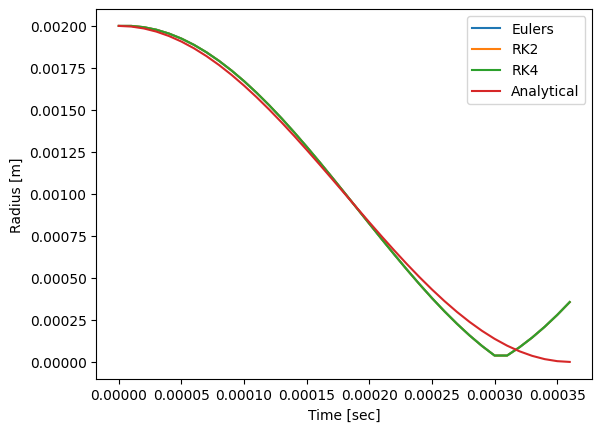
\includegraphics[scale=0.75]{out/dt_variance/Question_1/dt_1e-05/combined_graph.png}
    \caption{Simplified System - Radius vs Time for $\Delta\,t = 1e-05$ }
    \label{fig:part_1_big_step}
\end{figure}

\noindent As the $\Delta \, t$ value was decreased, the accuracy increased. Figure \ref{fig:part_1_solutions} shows all the solution methods approaching the analytical solution, such that they cannot be seen behind it.

\begin{figure}[H]
    \centering
    \begin{subfigure}[h]{0.495\textwidth}
        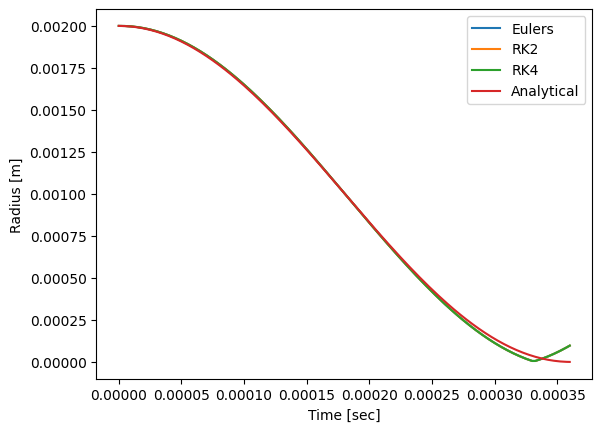
\includegraphics[width=\textwidth]{out/dt_variance/Question_1/dt_2.5e-06/combined_graph.png}
        \caption{Radius vs Time for $\Delta\,t = 2.5e-06$}
        \label{fig:part_1_2.5e-06}
    \end{subfigure}
    \hfill
    \begin{subfigure}[h]{0.495\textwidth}
        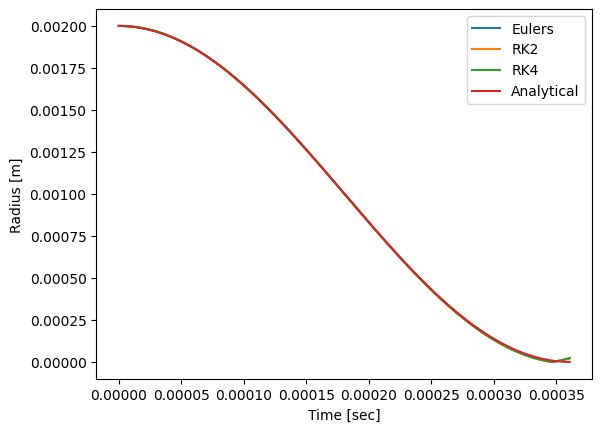
\includegraphics[width=\textwidth]{out/dt_variance/Question_1/dt_6.25e-07/combined_graph.png}
        \caption{Radius vs Time for $\Delta\,t = 6.25e-07$}
        \label{fig:part_1_6.25e-07}
    \end{subfigure}
    \vskip\baselineskip
    \begin{subfigure}[h]{0.495\textwidth}
        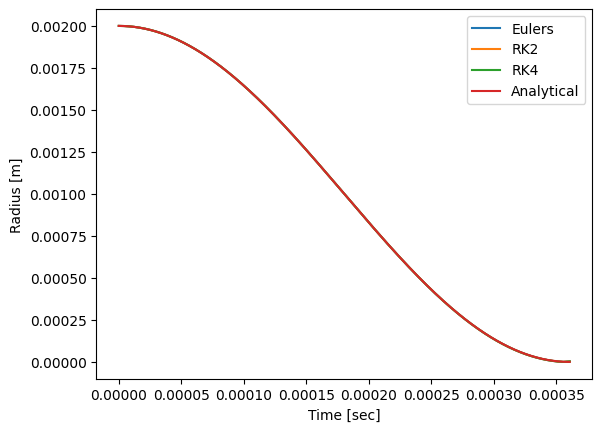
\includegraphics[width=\textwidth]{out/dt_variance/Question_1/dt_7.8125e-08/combined_graph.png}
        \caption{Radius vs Time for $\Delta\,t = 7.8125e-08$}
        \label{fig:part_1_7.8125e-08}
    \end{subfigure}
    \hfill
    \begin{subfigure}[h]{0.495\textwidth}
        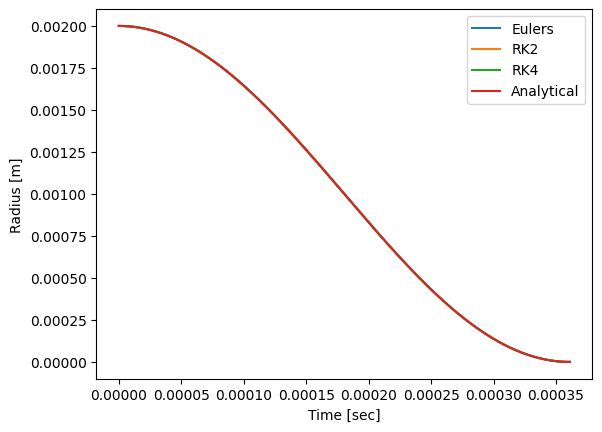
\includegraphics[width=\textwidth]{out/dt_variance/Question_1/dt_9.765625e-09/combined_graph.png}
        \caption{Radius vs Time for $\Delta\,t = 9.765625e-09$}
        \label{fig:part_1_9.765625e-09}
    \end{subfigure}
\caption{Simplified System - Solutions with different $\Delta \, t$ values}
\label{fig:part_1_solutions}
\end{figure}

From figure \ref{fig:part_1_solutions}, we can assume that a smaller $\Delta \, t$ leads to higher accuracy. In order to quantify the error for each method, the $R$ value was taken at $t=0.00034$ for each solution method. The $R$ value was then compared to the analytical solution and the error was marked in figure \ref{fig:part_1_error}. As similarly demonstrated in figure \ref{fig:part_1_solutions}, figure \ref{fig:part_1_error} shows that all the solution methods have the same amount of error when compared to the analytical solution; they are all identical to the RK4 solution's error which is visible in the plot. With respect to the analytical solution, the maximum error for all three methods has a magnitude of $1\times10^{-4}\, [m]$ which occurs when $\Delta\, t = 1.5\times10^{-5} \,[sec]$.

\begin{figure}[H]
    \centering
    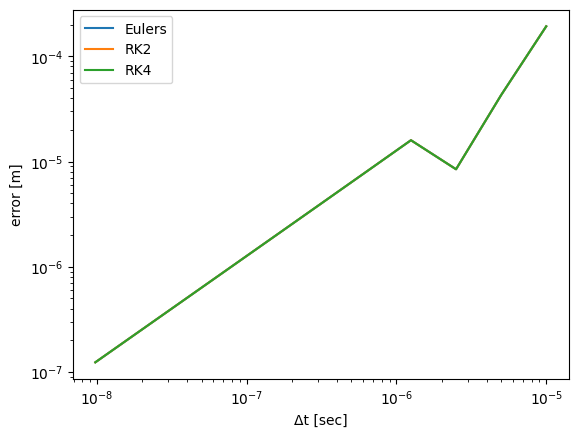
\includegraphics[scale=0.75]{out/error/Question_1/error.png}
    \caption{Simplified System - Error of Solving Methods}
    \label{fig:part_1_error}
\end{figure}

Furthermore, to quantify the accuracy of each solution method when solving the simplified ODE, the grid convergence of each method’s results is marked in Figure \ref{fig:part_1_r_at_t}. For each method, the $R$ value was taken at $t = 0.00034$ using each of the time steps from $\Delta\, t = 1.25\times 10^{-6}$ to $\Delta\, t = 9.765325 \times 10^{-9}$. Figure \ref{fig:part_1_r_at_t} shows that as $\Delta\, t$ decreases, the accuracy increased. As concluded earlier, the solution methods are almost identical. We can use the grid convergence to verify the solution methods' results against the actual result from the simplified ODE. Therefore, because all solution methods converge to approximately $R = 0.00002\, [m]$ at $t = 0.00034\, [sec]$, the actual result of the simplified ODE will approach the same solution.


\begin{figure}[H]
    \centering
    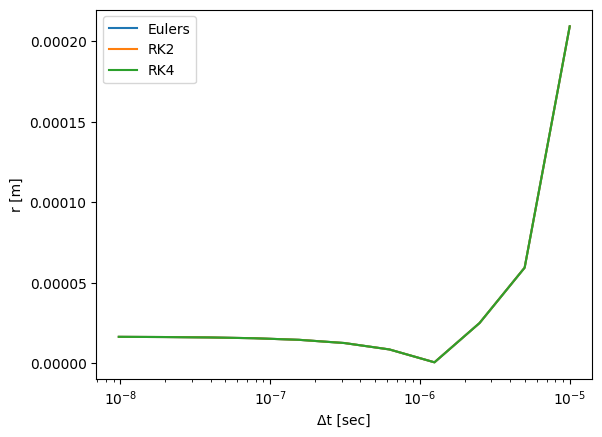
\includegraphics[scale=0.75]{out/error/Question_1/r_at_t.png}
    \caption{Simplified System - $R$ values at $t=0.00034$}
    \label{fig:part_1_r_at_t}
\end{figure}

% PART 2 ────────────────────────────────────────────────────────────────────────── 
\clearpage
\section{Rayleigh-Plesset Equation}

Now having a functional numerical solution method, the attention turns back to the original Rayleigh-Plesset equation \cite{rayleigh-eqn}. While the simplified solution provides some insight into how the bubble system acts, it does not provide very accurate values near the collapse. For this reason, the R.P. equation is far preferable.

\begin{equation}
    \label{eqn:part_2_rayleigh}
    \rho_l \left(R \dot R + \frac{3}{2}\dot R^2\right) = -P_0 -4 \mu \frac{\dot R}{R} - 2 \frac{\sigma}{R}
\end{equation}

\subsection{Bubble Energy}
An interesting thing to consider is how much energy is required to create these bubbles. If it is assumed that the forces of surface tension and fluid viscosity are ignored, and assumed that the bubble does not contain any vapour, the energy of formation of the bubble can be treated as work by displacement. 

\begin{equation}
    \label{eqn:part_2_general_work}
    W = \int_a^b P dV
\end{equation}

\noindent Assuming that the bubble forms in a body of water large enough that the height of fluid does not significantly change due to displacement, the pressure will be constant at any given depth. Substituting the constant P value and the volume of a sphere, we arrive at equation \ref{eqn:part_2_bubble_energy}.

\begin{subequations}
    \centering
    \begin{align}
        W &= \int_a^b \underbrace{P}_{\text{const.}} dV \notag\\
        W &= P \int_0^r dV \notag\\
        W &= P \, \Delta V \notag\\
        W &= P \, \frac{4}{3} \pi r^3 \label{eqn:part_2_bubble_energy} \\
        4.5280822 \times 10^{13}\, [J]&= 10810000\, [Pa] \times \frac{4}{3} \pi \left(100 \,[m]\right)^3 \label{eqn:part_2_energy}
    \end{align}
\end{subequations}

As shown by equation \ref{eqn:part_2_energy}, The energy for creation of a 100 meter vacuum bubble at 1000 meters of depth is on the same order of magnitude as the orbital kinetic energy of the International Space Station \cite{iss_velocity}\cite{iss_mass} or the Little Boy nuclear bomb dropped on Hiroshima \cite{little_boy_yield}. This is an incredible amount of energy. The only reasonable means of creating a vacuum bubble of this scale would be to detonate a nuclear warhead under the ocean.

\subsection{Numerical Solution}

In order to arrive at a numerical solution for the Rayleigh-Plesset equation, the same steps are followed as with the simplified ODE. The equation must first be converted to a system of first order ODEs and incremented over using a numerical method. Unfortunately, some aspects of this system make it more difficult to implement in software.

\subsubsection{Order Reduction} \label{sec:part_2_order_reduction}

Firstly, the system must be converted to a system of first order ODEs. Since the Rayleigh-Plesset equation is only second order, the same substitution can be used as is outlined in section \ref{sec:part_1_order_reduction} and equation \ref{eqn:part_1_order_reduction}. Equation \ref{eqn:part_2_order_reduction} shows the substitution and construction of the system of equations.

\begin{subequations}
    \label{eqn:part_2_order_reduction}
    \centering
    \begin{gather}
        \rho_l \left(R \dot R + \frac{3}{2}\dot R^2\right) = -P_0 -4 \mu \frac{\dot R}{R} - 2 \frac{\sigma}{R} \\
        \text{Substitute:} \quad \dot P = \ddot R \, , \quad P = \dot R\\
        \begin{aligned}
            \rho_l \left(R \dot P + \frac{3}{2}P^2\right) &= -P_0 - 4 \mu \frac{P}{R} - 2 \frac{\sigma}{R} \notag \\
            \rho_l R \dot P + \frac{3}{2} \rho_l P^2 &= -P_0 - 4 \mu \frac{P}{R} - 2 \frac{\sigma}{R} \notag
        \end{aligned}\\
        \dot P = \frac{-P_0 - 4 \mu \frac{P}{R} - 2 \frac{\sigma}{R} - \frac{3}{2}\rho_l P^2}{\rho_l P} \notag \\
        {\large\therefore} \qquad R =
        \begin{cases}
            \dot P = \frac{-P_0 - 4 \mu \frac{P}{R} - 2 \frac{\sigma}{R} - \frac{3}{2}\rho_l P^2}{\rho_l P} \\
            \dot R = P
        \end{cases} \label{eqn:part_2_order_reduction_system}
    \end{gather}
\end{subequations}

\noindent Notably, the $\dot P$ value is defined to be a function of a couple of terms, including $-4\mu \frac{P}{R}$ and $-2 \frac{\rho}{R}$. These two terms present an issue in that they approach infinity as the bubble's radius approaches zero. These issues are handled more directly in section \ref{sec:part_2_software_impl} with the software implementation. 

\subsubsection{Solution Methods}

Looking at the results in section \ref{sec:part_1_analysis}, It is clear that, while it requires more computational time, the RK4 method is the most accurate of the solution methods. For this reason, the RK4 method is used to solve the system. In order to observe the behaviour of the other solution methods, both Eulers Method and the RK2 method are also tested.

\subsubsection{Software Implementation} \label{sec:part_2_software_impl}

As mentioned at the end of section \ref{sec:part_2_order_reduction}, the $-4\mu \frac{P}{R}$ and $-2 \frac{\rho}{R}$ terms from the ODE system in equation \ref{eqn:part_2_order_reduction_system} present an issue as $R$ approaches zero. The solution to this problem was to limit the absolute values of $\dot R$ and $\dot P$. This allows the system to operate close enough to the true mathematical model without requiring incredibly large float values to remain accurate. While this change does effect the slope greatly, the range of $t$ values for which $\dot R$ and $\dot P$ are this large is very very small. Through experimentation, it was determined that a reasonable slope limiting value was $10^6$. This value seemed to provide the most consistent results. The slope value was limited using the \texttt{numpy.clip} function in Python; The placement of which can be found in listing \ref{lst:slope_limiting} on line \ref{code:np_clip_call} in the solver class.

\setcounterref{lstlinereffirst}{code:rk4_start}
\setcounterref{lstlinereflast}{code:rk4_end}
\lstinputlisting[title=\texttt{\scriptsize Slope Limiting with \texttt{numpy.clip} in line \ref{code:np_clip_call}},
                 caption=Slope Limiting with \texttt{numpy.clip} in line \ref{code:np_clip_call} | Solvy\_boi.py,
                 label=lst:slope_limiting,
                 firstline=\thelstlinereffirst,
                 lastline=\thelstlinereflast,
                 firstnumber=\thelstlinereffirst]{./Solvy_boi.py}

The Rayleigh-Plesset equation created another issue. As the system approaches zero, the collapse speed increases and eventually the system arrives at $R=0$ at this point, referred to as the singularity, there is an incredible pressure spike. For simplification in this report, it can be assumed that at the singularity, all the inward pointed velocities instantly reverse and point outward. While this effect could be well estimated in software using a more complex Time Of Impact (TOI) algorithm, a more simple approach was used for this model. The iteration functions each make use of sign inversion correction. After the $i+1$ values are calculated for each iteration, the variable of consequence (in this case, $R$) is checked for if the sign has changed (+/-). If the sign has changed, the values for $i$ are restored and the other values ($P$) are multiplied by $-1$. This forces $R$ to always be a positive value, but reduces the precision. The maximum error for this case is a function of the time step of the iteration. As the time step decreases, so does the potential error near $R=0$. The implementation of the sign inversion correction is shown in listing \ref{lst:sign_inversion}.

\setcounterref{lstlinereffirst}{code:sign_inversion_start}
\setcounterref{lstlinereflast}{code:sign_inversion_end}
\lstinputlisting[title=\texttt{\scriptsize Sign Inversion Correction},
                 caption=Sign Inversion Correction | Solvy\_boi.py,
                 label=lst:sign_inversion,
                 firstline=\thelstlinereffirst,
                 lastline=\thelstlinereflast,
                 firstnumber=\thelstlinereffirst]{./Solvy_boi.py}

The implementation of the solver class is shared between the solutions of the simplified ODE and the Rayleigh-Plesset equation. These functions are used in both cases, but only really effect the outcome of the Rayleigh-Plesset equation, where the slope has the potential to exceed $10^6$ and the radius is liable to dip below 0.

\subsection{Solution Analysis}

The R.P. system was again solved using a range of time steps: the largest being $1\times10^{-2}$ and the smallest being $9.765625\times10^{-6}$. These time steps where selected over a logarithmic range, with each step being half of the previous. This ensured that certain time steps are always present in the output. This is useful for quantifying error in Figure \ref{fig:part_2_error} further down.

Unlike the simplified ODE, for larger $\Delta \, t$ values, the R.P. system was less stable and resolved with lower accuracy when compared with the smaller time steps. Additionally, Figure \ref{fig:part_2_solutions} demonstrates that, at larger time steps, the RK4 solutions have a higher accuracy and stability than the RK2 solutions. This coincides with the results in section \ref{sec:part_1_analysis}. 

The data also highlights the relationship between the time step used to solve the R.P. equation and the time observed between two neighbouring collapses. For $\Delta \, t > 6.25\times10^{-4}$, the R.P. system was unstable and produced multiple collapses at a higher and sporadic frequency as time increased. However, as concluded from the simplified ODE, as $\Delta \, t$ decreased, a higher accuracy was produced as both the number and frequency of bubble collapses over time becomes consistent. Figures \ref{fig:part_2_0.000625} and \ref{fig:part_2_9.765625e-06} illustrate the high accuracy achieved by the RK4 solution once the time step is sufficiently small. 

\begin{figure}[H]
    \centering
    \begin{subfigure}[h]{0.495\textwidth}
        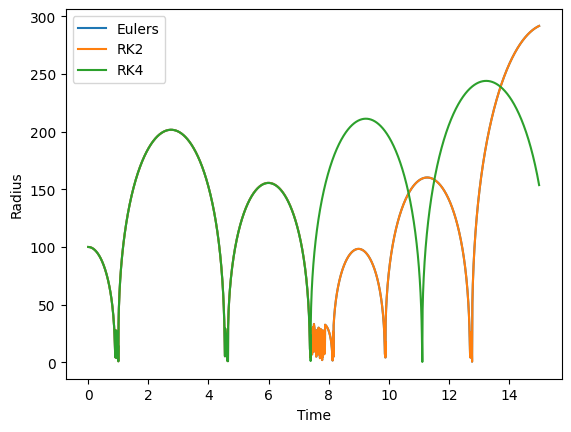
\includegraphics[width=\textwidth]{out/dt_variance/Question_2/dt_0.005/combined_graph.png}
        \caption{Radius vs Time for $\Delta\,t = 0.005$}
        \label{fig:part_2_0.005}
    \end{subfigure}
    \hfill
    \begin{subfigure}[h]{0.495\textwidth}
        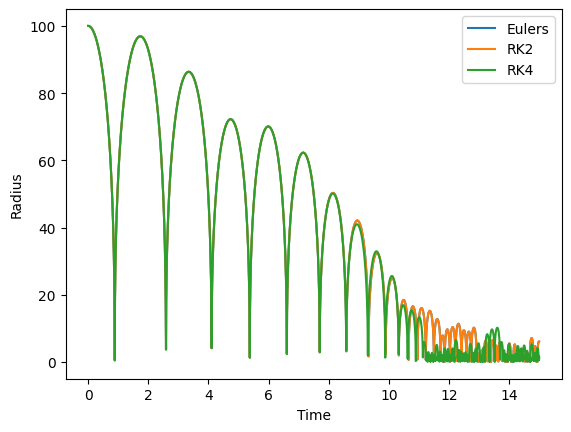
\includegraphics[width=\textwidth]{out/dt_variance/Question_2/dt_0.00125/combined_graph.png}
        \caption{Radius vs Time for $\Delta\,t = 0.00125$}
        \label{fig:part_2_0.00125}
    \end{subfigure}
    \vskip\baselineskip
    \begin{subfigure}[h]{0.495\textwidth}
        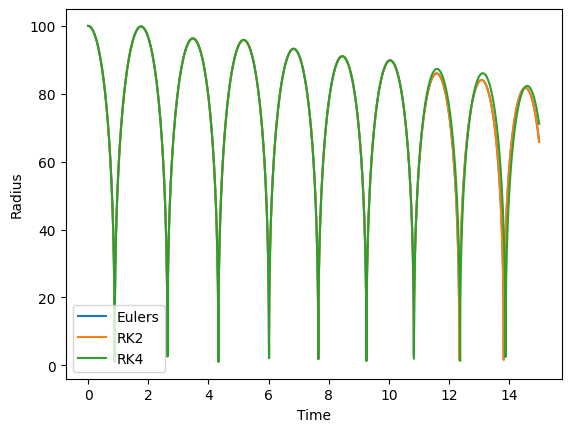
\includegraphics[width=\textwidth]{out/dt_variance/Question_2/dt_0.000625/combined_graph.png}
        \caption{Radius vs Time for $\Delta\,t = 0.000625$}
        \label{fig:part_2_0.000625}
    \end{subfigure}
    \hfill
    \begin{subfigure}[h]{0.495\textwidth}
        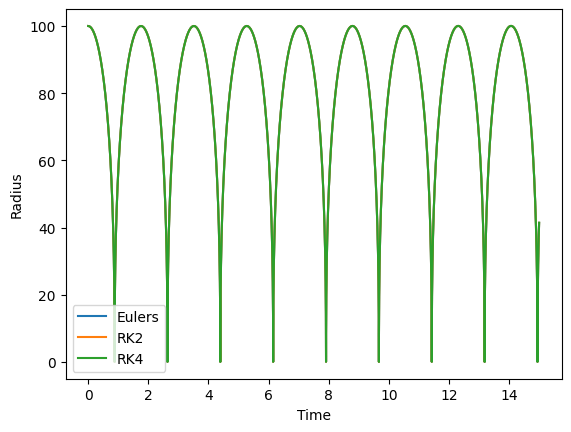
\includegraphics[width=\textwidth]{out/dt_variance/Question_2/dt_9.765625e-06/combined_graph.png}
        \caption{Radius vs Time for $\Delta\,t = 9.765625e-06$}
        \label{fig:part_2_9.765625e-06}
    \end{subfigure}
\caption{Rayleigh-Plesset System - Solutions with different $\Delta \, t$ values}
\label{fig:part_2_solutions}
\end{figure}

In order to quantify error (when solving the full R.P. equation) between the methods of Euler, RK2, and RK4, the $R$ value was taken at $t = 14$ for each solution method. Each solution's respective $R$ value was then compared to the $\Delta t_{\text{min}}$ RK4 solution and the error was marked in Figure \ref{fig:part_2_error}. It is interesting to note the slight differences of error between RK2 and RK4, which are more apparent when solving the full R.P. equation as opposed to the simplified ODE; in Section \ref{sec:part_1_analysis} both methods' error are nearly indistinguishable from each other. However, all the solution methods have a lower error for the R.P. equation at the same respective $\Delta \, t$ than they had with solving the simplified ODE. 

\begin{figure}[H]
    \centering
    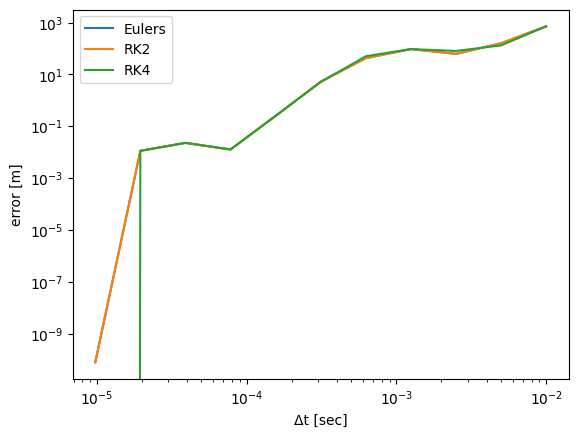
\includegraphics[scale=0.75]{out/error/Question_2/error.png}
    \caption{Rayleigh-Plesset System - Error of Solving Methods}
    \label{fig:part_2_error}
\end{figure}

Furthermore, to quantify the accuracy of each solution method when solving the R.P. equation, the grid convergence of each method's results is marked in Figure \ref{fig:part_2_r_at_t}. For each method, the $R$ value was taken at $t$ = 14.0 using each of the time steps from $\Delta\,t = 0.01$ to $\Delta\,t = 9.765625\times10^{-6}$. Figure \ref{fig:part_2_r_at_t} shows that as $\Delta\, t$ decreases, the value of $R$ converges to 100 metres. As concluded earlier, the solution of RK4 becomes more accurate as the time step used becomes smaller. Since we do not have the analytical solution to the full R.P. equation, we can use the grid convergence to determine if the real solution will converge. Therefore, because all solution methods converge to $R$ = 100m at $t$ = 14.0 seconds, the actual result of the R.P. equation will approach the same solution.

\begin{figure}[H]
    \centering
    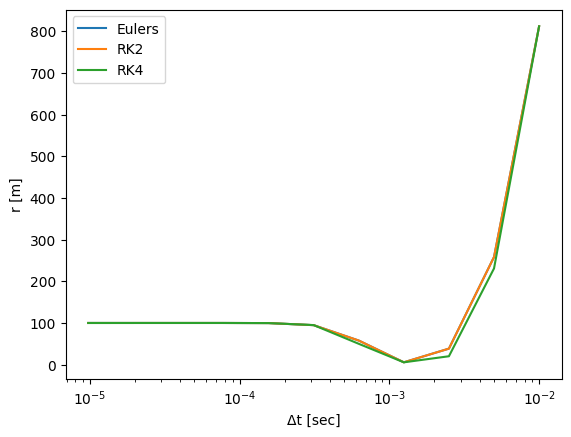
\includegraphics[scale=0.75]{out/error/Question_2/r_at_t.png}
    \caption{Rayleigh-Plesset System - $R$ values at $t=14.0$}
    \label{fig:part_2_r_at_t}
\end{figure}

\subsection{Radius Variation}

In order to observe the behaviour of smaller vacuum bubbles, the system was solved for a range of different radiuses: 0.1, 1, 10, and 100 meters. The results of which are shown in the figure \ref{fig:size_variance}.

\begin{figure}[H]
    \centering
    \begin{subfigure}[h]{0.495\textwidth}
        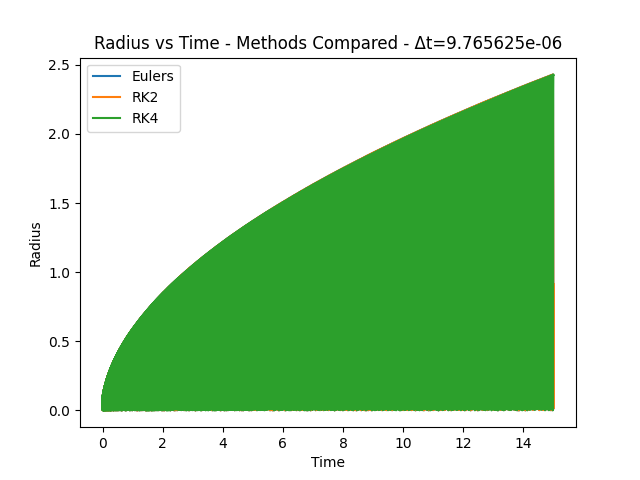
\includegraphics[width=\textwidth]{out/size_variance/Question_2/0.1/dt_9.765625e-06/combined_graph.png}
        \caption{Radius vs Time for $R_0 = 0.1\, [m]$}
        \label{fig:radius_0.1}
    \end{subfigure}
    \hfill
    \begin{subfigure}[h]{0.495\textwidth}
        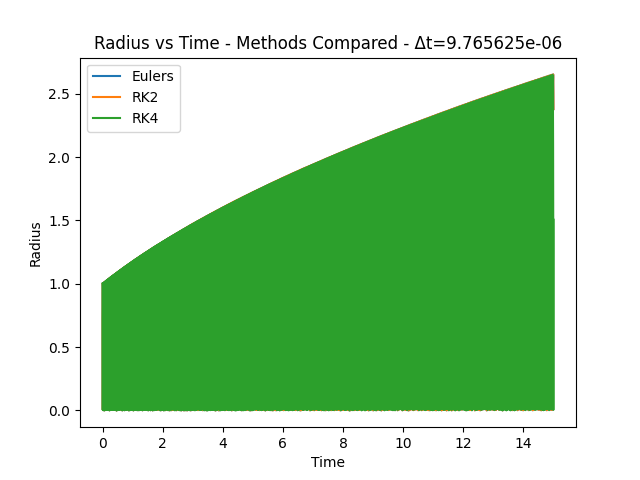
\includegraphics[width=\textwidth]{out/size_variance/Question_2/1/dt_9.765625e-06/combined_graph.png}
        \caption{Radius vs Time for $R_0 = 1\, [m]$}
        \label{fig:radius_1}
    \end{subfigure}
    \vskip\baselineskip
    \begin{subfigure}[h]{0.495\textwidth}
        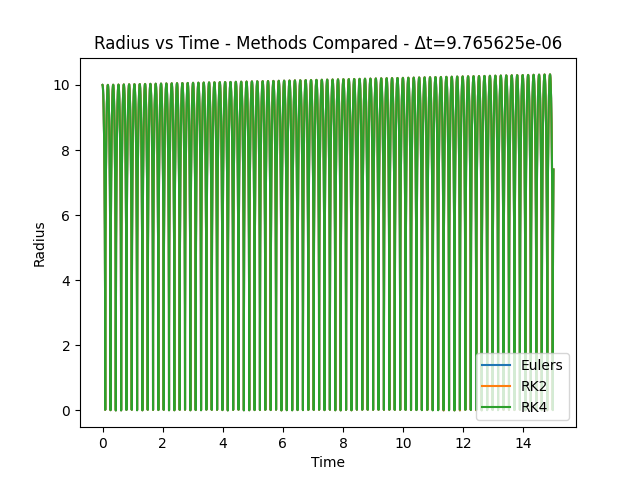
\includegraphics[width=\textwidth]{out/size_variance/Question_2/10/dt_9.765625e-06/combined_graph.png}
        \caption{Radius vs Time for $R_0 = 10\, [m]$}
        \label{fig:radius_10}
    \end{subfigure}
    \hfill
    \begin{subfigure}[h]{0.495\textwidth}
        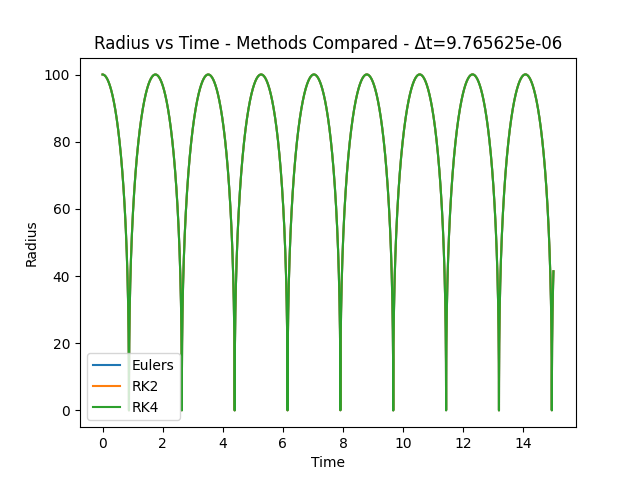
\includegraphics[width=\textwidth]{out/size_variance/Question_2/100/dt_9.765625e-06/combined_graph.png}
        \caption{Radius vs Time for $R_0 = 100\, [m]$}
        \label{fig:radius_100}
    \end{subfigure}
\caption{Rayleigh-Plesset System - Solutions with different $R_0$ values}
\label{fig:size_variance}
\end{figure}

The most obvious thing about the graphs is that, as $R_0$ increases, so does the period of oscillation. Table \ref{tbl:part_2_t_star} shows that the time of the first collapse varies almost linearly with the initial radius. Due to the precision of this numerical solver, it is assumed that the variation is error, and that the values are linearly related.

\begin{table}[H]
    \centering
    \caption{First Collapse Time vs Initial Radius}
    \label{tbl:part_2_t_star}
    \begin{tabular}{|c|l|}
        \hline
        $R_0 \, [m]$ & \multicolumn{1}{|c|}{$T^*_1 \, [sec]$} \\
        \hline
        0.1 & 0.0009765625 \\
        1 & 0.008984375000000001 \\
        10 & 0.08826171875 \\
        100 & 0.8790625 \\
        \hline
    \end{tabular}
\end{table}

Additionally, in figure \ref{fig:size_variance}, it is easy to see that the smaller $R_0$ values create errors with the current solver implementation. This is likely due to the accumulation in the very small error at the rebound point when the sign inversion correction from section \ref{sec:part_2_software_impl} is enacted. Table \ref{tbl:part_2_rebound} shows the $R$ and $\dot R$ immediately before and after the sign inversion kicks in.

\begin{table}[H]
    \centering
    \caption{Singularity Rebound Amplification}
    \label{tbl:part_2_rebound}
    \begin{tabular}{|c|l|l|l|}
        \hline
        $i$ & \multicolumn{1}{|c|}{$t$} & \multicolumn{1}{|c|}{$\dot R$} &  \multicolumn{1}{|c|}{$R$}\\
        \hline
        98 & 0.00095703125 & -366.564575925969 & 0.00642150348534173 \\
        99 & 0.000966796875 & -376.330200925969 & 0.00284177129856469 \\
        100 & 0.0009765625 & 376.330200925969 & 0.00284177129856469 \\
        101 & 0.000986328125 & 366.564575925969 & 0.00651687091698236 \\
        \hline
    \end{tabular}
\end{table}

\noindent Between $i=99$ and $i=100$, the new state is calculated to have $R < 0$. This causes the slope to be inverted for the next state point. The issue arises due to how the slope is handled. The $R$ value is calculated for $i=98 \, \rightarrow i=99$ using the $R$ and $\dot R$ of $i=98$, but when it rebounds and takes the first increasing step of $i=100 \, \rightarrow i=101$ using the $R$ and $\dot R$ of $i=100$. Looking at these values, it is evident that $\dot R_{i=98} < -\dot R_{100}$. This subtle amplification is not significant when there are small number of rebound events, such as when a large $R_0$ is used. But, as the frequency of rebounds increases, the effect becomes far more pronounced. For future implementations, this issue could be resolved by storing the $\dot R$ value for 1 previous state, allowing the sign inversion correction to utilize the previous slope value instead of the current. This should remove the amplification and provide more consistent data. Unfortunately, this could not be implemented in time to have new data calculated.

% BIBLIOGRAPHY ──────────────────────────────────────────────────────────────────── %
\clearpage
\bibliographystyle{plain} % We choose the "plain" reference style
\bibliography{references} % Entries are in the references.bib file

% APPENDIX ──────────────────────────────────────────────────────────────────────── %
\clearpage
\section{Appendix} \label{appendix}

\subsection{Equations} \label{appendix_equations}

% Part 1 Analytical Solution derivation
\begin{subequations}
    \label{eqn:anl_deriv}
    \noindent \underline{\bf Primary ODE simplification}
    \centering
    \begin{gather}
        \ddot R + \lambda^2 \left(R - R_0\right) = \frac{-3}{2} \frac{P_0}{\rho_l R_0}, \quad \text{where} \, \lambda^2 = \frac{3 P_0}{\rho_l R_0^2} \\
        \downarrow \notag \\
        \ddot R + \lambda^2 R - \lambda^2 R_0 = \frac{-3}{2}\frac{P_0}{\rho_l}{R_0} \notag \\
        \ddot R + \underbrace{\lambda^2 P}_{\text{const. }j} = \underbrace{\frac{-3}{2}\frac{P_0}{\rho_0 R_0} - \lambda^2 R_0}_{\text{const. }k} \notag \\
         \begin{array}{c|c}
            \begin{aligned}
                j &= \lambda^2 \notag\\
                j &= \frac{3 P_0}{\rho_l R_0^2} \notag
            \end{aligned}
            &
            \begin{aligned}
                k &= -\frac{3}{2}\frac{P_0}{\rho_0 R_0} - \lambda^2 R_0 \notag \\
                k &= -\frac{3}{2}\frac{P_0}{\rho_l R_0} - \frac{3 P_0}{\rho_l R_0} \notag \\
                k &= -\frac{9}{2}\frac{P_0}{\rho_l R_0} \notag
            \end{aligned}
         \end{array} \notag \\
        \therefore \quad \ddot R + jR = k \, , \quad \text{where} \, j = \lambda^2 = \frac{3 P_0}{\rho_l R_0^2} \quad \& \quad k = -\frac{9}{2}\frac{P_0}{\rho_l R_0}
    \end{gather}
    
    \underline{\bf Homogeneous Solution}
    \begin{gather}
        a \ddot R + b \dot R + c R = 0 \notag \\
        a=1 \, , \quad b = 0 \, , \quad c=j \notag \\
        R_h(t) = e^{\lambda_h t} \, , \quad \text{where } \lambda_h = \frac{-b  	\pm \sqrt{b^2 - 4ac}}{2a} \notag \\
        \lambda_h = \frac{0 \pm \sqrt{0 - 4(1)(j)}}{2(1)} \notag \\
        \begin{aligned}
            \text{Since non-real solution}: & \quad R_h(t) = c_a e^{\alpha t} \cos(\beta t) + c_b e^{\beta t}\sin(\beta t) \notag \\
            \text{where}, & \quad \lambda_{h_p} = \alpha + i \beta \, , \quad \lambda_{h_p} = \alpha + i \beta \notag \\
            \text{and}, & \quad \alpha = 0 \, , \quad \beta = \sqrt{j} \notag
        \end{aligned} \\
        \therefore \quad R_h(t) = c_a \cos \left(t\sqrt{j}\right) + c_b \sin \left(t\sqrt{j}\right)
    \end{gather}
    
    \underline{\bf Particular Solution}
    \begin{gather}
        \text{Since RHS is const., no derivatives needed:} \notag \\
        R_p(t) = c_0 \\
        \text{Substitute to find } c_0 \, \text{:} \notag \\
        \ddot R_p + j R_p = k \notag \\
        (0) + j (c_0) = k \notag \\
        c_0 = \frac{k}{j} = \frac{-\frac{9}{2}\frac{P_0}{\rho_l R_0}}{\frac{3 P_0}{\rho_l R_0^2}} = \frac {1}{2} R_0
    \end{gather}
    
    \underline{\bf General Solution}
    \begin{gather}
        R(t) = R_h(t) + R_p(t) \notag \\
        R(t) = c_a \cos\left(t\sqrt{j}\right) + c_b \sin\left(t\sqrt{j}\right) + \frac {1}{2} R_0 \\
        R(t) = c_a \cos\left(t\sqrt{\frac{3 P_0}{\rho_l R_0^2}}\right) + c_b \sin\left(t\sqrt{\frac{3 P_0}{\rho_l R_0^2}}\right) + \frac {1}{2} R_0
    \end{gather}
    
    \underline{\bf Initial Value Solution}
    \begin{gather}
        \begin{array}{c|c}
            \begin{aligned}
                R(t) &= c_a \cos\left(t\sqrt{j}\right) + c_b \sin\left(t\sqrt{j}\right) + \frac {1}{2} R_0 \notag \\
                R(0) &= c_a \cos\left((0)\sqrt{j}\right) + c_b \sin\left((0)\sqrt{j}\right) + \frac {1}{2} R_0 \notag \\
                0.002 &= c_a (1) + c_b (0) + \frac {1}{2} (0.002) \notag \\
                c_a &= 0.002 - \frac{1}{2} 0.002 = 0.001 \notag
            \end{aligned} \notag
            &
            \begin{aligned}
                \dot R(t) &= -c_a \sqrt j \, \sin\left(t\sqrt{j}\right) + c_b \cos\left(t\sqrt{j}\right) \notag \\
                \dot R(0) &= -c_a \sqrt j \, \sin\left((0)\sqrt{j}\right) + c_b \cos\left((0)\sqrt{j}\right) \notag \\
                0 &= -c_a \sqrt j \, (0) + c_b (1) \notag \\
                c_b &= 0 \notag
            \end{aligned} \notag
        \end{array} \notag \\
        j = \frac{3 P_0}{\rho_l R_0^2} = \frac{ 3 \times 100981}{1000 \times 0.002^2} = 7.573575 \times 10^7 \notag \\
        \sqrt{j} = \sqrt{7.573575 \times 10^7} = 8702.629 \notag \\
        R(t) = 0.001 \, \cos\left(8702.629 t \right) + 0.001
    \end{gather}
\end{subequations}

\clearpage
\subsection{Full Code Listings}

% Solvy_boi.py
\lstinputlisting[title=\texttt{\scriptsize Solvy_boi.py},
                 caption=ODE Solver Object | Solvy\_boi.py,
                 label=lst:solvy_boi_source]{./Solvy_boi.py}
\clearpage

% Question_1.py
\lstinputlisting[title=\texttt{\scriptsize Question_1.py},
                 caption=Question 1 Runner | Question\_1.py,
                 label=lst:q1_source]{./Question_1.py}
\clearpage

% Question_2.py
\lstinputlisting[title=\texttt{\scriptsize Question_2.py},
                 caption=Question 2 Runner | Question\_2.py,
                 label=lst:q2_source]{./Question_2.py}
\clearpage

% Auto_runner.py
\lstinputlisting[title=\texttt{\scriptsize Auto_runner.py},
                 caption=Auto Runner | Auto\_runner.py,
                 label=lst:auto_runner_source]{./Auto_runner.py}
\clearpage

% \bibliographystyle{abbrv}
% \bibliography{main}

\end{document}
